% ======= Welcome to HCoV Skills Workshop 1 =======
%
% For each task in the workshop, use "Think-Pair-Share":
% 1. *Think* about the task on your own;
% 2. Discuss your thoughts in a *pair* (or triple);
% 3. *Share* your pair's thoughts with the rest of your table and produce a group answer.
% 
% When the whole table is working together, one person
% should share their screen on the monitor so everyone
% can see easily.
%
% You may also want to Share the Overleaf project
% with the others in your group to collaborate.
%
% You should read through this source window to see the
% full instructions for the workshop.
%
% In this workshop we will do some small-scale writing
% exercises and cover some basics of using LaTeX.
%
\documentclass{UoESoMworkshop}
\title{HCoV Skills Workshop 1}

% Replace A, B, C, D below with the names of your group members.
% Then click Recompile (or press Ctrl+S).
\author{A, B, C, D}

\begin{document}
\maketitle

\section{Communication exercises}

Below are two attempts to describe Figure~\ref{fig:completeGraph} in such a way that someone else could reconstruct the figure from just the description.

\begin{figure}[h]
    \centering
    
\includegraphics[width=0.35\textwidth]{d9}
    \caption{A figure to be described}
    \label{fig:completeGraph}
\end{figure}

\begin{quote}
``The figure consists of a circle on the perimeter of which 
are marked five equally spaced points, one of which is coloured black with the remaining coloured blue. 
Each of these five points is joined to the two points furthest from it by a line segment.''
\end{quote} 

\noindent Or I might try to do it by naming the points: 
\begin{quote}
``The figure consists of a circle on the perimeter of which are marked five equally spaced points $A,B,C,D,E$ in order. 
(The points could be the vertices of a regular pentagon.) Four points are coloured blue and the fifth point is coloured black.
As well as the circle, the diagram contains the line segments $AC$, $BD$, $CE$, $DA$ and $EB$.''
\end{quote} 


\begin{exercise}[10 min]
On your own, take 3 minutes to consider each of the above descriptions. Which do you think is better given that the aim was for someone else to be able to reconstruct the figure from just the description? In what situations might each description be better than the other? Can you improve the descriptions?

Now discuss your views with the rest of your group.
\end{exercise}


\begin{exercise}[15 min]
% Write a description of Figure~\ref{fig:d7}. Start with your own draft and then agree a final version. The aim is for someone else to be able to reconstruct the figure unambiguously from the description.
\end{exercise}

\begin{figure}[h]
    \centering
    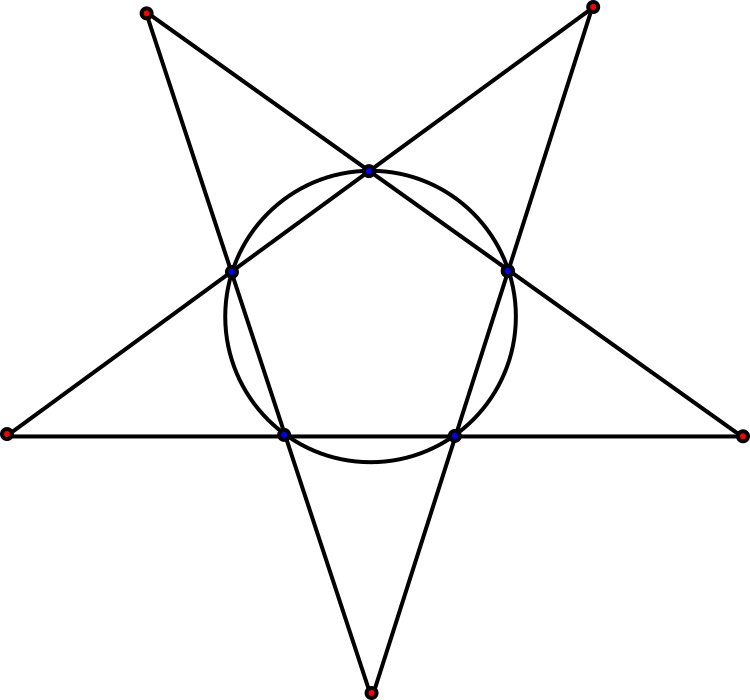
\includegraphics[width=0.6\textwidth]{pent}
    \caption{A figure for you to describe}
    \label{fig:d7}
\end{figure}

% == Type your description in here ===

% ====================================


\section{Correct the \LaTeX{} code}

\begin{exercise}[15 min]
Correct the LaTeX in this section according to the comments in the source code.
